\chapter{Objective}
\label{cha:second_intro}
\definechapterdirectory{src/second_intro}

The general objective of this thesis is to provide tools that will expose cache
coherence interference to an applicant seeking the certification of system with
multi-core processor, thereby contributing to the resolution of the
\textit{Resource Usage 3} requirement. Indeed, that requirement asks that the
applicant identifies all interference and its impact on the applications.

As the necessary notions have now been introduced, the problem statement from
Section~\ref{sec:intro:prob_statement} and the proposed solution can be
presented in more details. Thus, this chapter clarifies the scope of this
thesis and provides an explanation of how its contributions form a framework
that exposes cache coherence interference.

\stopallthesefloats
\section{Tasks Required of the Applicant}
To fulfill the \textit{RU3} objective, the applicant has to catalog all
interference channels, as well as all interference, and to mitigate them so that
they do not prevent the applications from otherwise fulfilling other
requirements. To determine where the interference is and how much of an impact
they could potentially have, an understanding of the architecture's mechanisms
is required. When the mechanisms that generate them are not removed all
together, the applicant must be able to quantify their impact on the running
software.

\subsection{Coherence Protocol Identification}
\label{aaa:identification}
Ideally, the solution would simply be to consult the architecture's
documentation, where the mechanisms would be described in details and,
hopefully, so would all interference inducing behaviors. However, actual
documentation for COTS processors do not generally include details on cache
coherence. This is the first issue addressed in this thesis: how can one be sure
of their understanding of the architecture's cache coherence mechanisms?
On this topic, the contribution this thesis makes is to point out a missing
preliminary step, and propose a strategy for it. Indeed, instead of focusing on
the already resolved issue of measuring the time required to perform an access,
or the bandwidth such accesses would have, the issue of incorrect assumptions on
the architecture's cache coherence mechanisms is addressed. In effect, because
the documentation of the implemented cache coherence mechanisms is not precise,
there is a strong risk of mismatch between what the architecture actually
performs and what is being tested, for why would one test the performance of
something they understand not to be present?

For example, if a \textit{MESI} architecture was benchmarked as if it were a
\textit{MSI} one, the interference generated by having two caches each perform
an initial read on a memory would, for one of the two caches, not be the same as
with a true \textit{MSI} architecture. Not realizing this would lead the
applicant to wrongly characterize the architecture. They could incorrectly
underestimate the cost of simultaneous reading, if the measures happened to be
done on the second cache to complete reading, as the data would then be provided
by the first cache. Since this is happens only in special cases with the
\textit{MESI} protocol, to consider this measure representative of the general
case of parallel reading would lead to a completely incorrect analysis of the
effects of interference. Since these special cases are not found within the
\textit{MSI} cache protocol, the applicant would not know to be wary of them.

Ensuring that the architecture's cache coherence mechanisms have properly been
identified and their characteristics measured is a necessary step for the
analysis of the architecture. It is however not sufficient to infer what
interference the architecture's mechanisms will generate, nor how it will
affect the execution of the applications.

\subsection{Measuring the Impact of Interference of the Software}
\begin{definition}[Impact of Interference]
\label{sec:impact_of_interference}
The impact of an interference is a quantification of the temporal effects of
interference on an application's execution. More precisely, it is the amount of
additional CPU cycles required to execute a given fragment of the application
compared its execution in isolation.
\end{definition}

\begin{figure}[hbt!]
\begin{center}
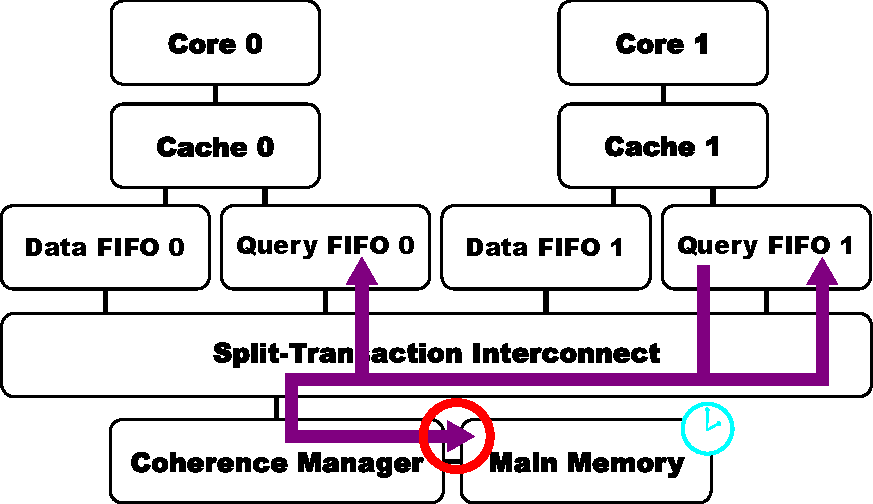
\includegraphics[width=0.6\textwidth]{\chapterdirectory/figure/demo_arch1.pdf}
\end{center}
\caption{Second Example of Interference}
\label{fig:second_intro:interference_example2}
\end{figure}

\begin{example}[Impact of Interference]
The interference from Example~\ref{ex:second_intro:interference}, by itself, may
not be noticeable by \textit{Core 1} if it lasts less than a cycle. However, an
impact could be measured in a follow-up interference: once \textit{Cache 0}'s
query reaches the main memory, it stays busy for an appreciable amount of time
before becoming available once again (see
Figure~\ref{fig:second_intro:interference_example2}). Here also, \textit{Cache
1}'s query ends up delayed. In effect, if the main memory stays busy for 12 CPU
cycles before \textit{Cache 1}'s query is considered, then the impact of that
interference is the 12 CPU cycles delay.
\end{example}

Even when the architecture's mechanisms have been fully identified, predicting
the impact of interference on the execution of programs is not an issue
currently resolved by the existing literature. Restricting this issue to caches
in which coherence has been disabled still does not lead to a perfect solution.
Indeed, this was already problematic in single core systems in which multiple
applications share a same cache. The issue being that some aspects of the
architecture will still remain slightly ambiguous, and so the exact order in
which events occur cannot be determined.  Depending on the placement and
replacement policies of the cache, this makes it difficult to know the content
of the cache at any given time.  Cache coherence adds to the number of events
that can occur, and make the content of other caches decide whether events
occur, thus tremendously complexifying the issue. Ignoring the effects of
such mechanisms would quickly lead to either incorrect or unusable execution
time estimations, as any memory access would have a seemingly random temporal
cost as the then invisible coherence states would influence it. The existing
literature offers compromises: either analyzing strategies that will yield
overly pessimistic WCET, or restrictions to eliminate sources of interference so
that their effects need not be taken into account.  The available analysis
strategies do not address cache coherence. Some of the approaches using
restrictions do take cache coherence into account, but only through hardware
modifications, which is not deemed acceptable in an aeronautical context. This
thesis proposes an approach to analyze the effects of cache coherence. The idea
is to have an accurate representation of all mechanisms that are known and use
formal methods to ensure all possible behaviors of the mechanisms for which
ambiguities remain are explored.

\stopallthesefloats
\section{Proposed Solution}
In effect, this thesis proposes to tackle the issue of interference generated by
cache coherence by first ensuring complete understanding of the architecture's
cache coherence mechanisms through the proposed identification strategy, then
using existing approaches to measure the timing characteristics of these
mechanisms, to finally use formal methods on a model based on what is presented
in this thesis in order to infer the effects of the interference on the running
software.

\subsection{Hypotheses and Limitations}
\label{sec:thesis_hypotheses}
This section presents the hypotheses made on the context in order to limit the
scope of this thesis, as well as the reason behind these limitations and, when
applicable, how these could be removed in future works.

The first scope restrictions stem from the aeronautical context. Indeed:
\begin{itemize}
\item Only COTS architectures are considered. The use of self-made hardware is
not deemed acceptable in critical systems such as avionics.
\item Uses cache coherence. Using multi-core processors without cache coherence
prevents any gain they would otherwise provide over single-core processors when
running application with parallel processing.
\item Snooping-based cache coherence. This is the more common approach to cache
coherence in COTS, and thus makes for a good starting point. Extending this
thesis to also handle directory-based cache coherence would require the creation
of a different architecture model.
\end{itemize}

Other restrictions are more related to what the thesis' time constraints
permitted. The focus stayed on cache coherence itself, since this is what the
existing literature consistently avoids. Thus, elements that are already
explored in other numerous works have not been expended upon past the bare
minimum. An example of architecture complying with these restrictions can
be seen in Figure~\ref{fig:second_intro:typical_arch}.

\begin{figure}[hbt!]
\begin{center}
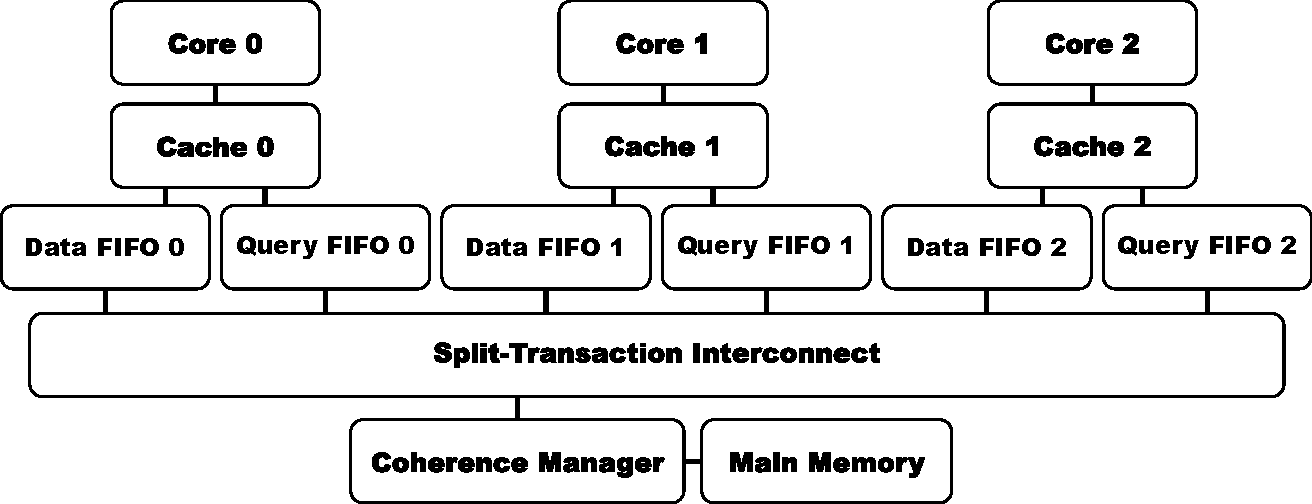
\includegraphics[width=\textwidth]{\chapterdirectory/figure/typical_arch3.pdf}
\end{center}
\caption{Typical profile of the targeted architecture}
\label{fig:second_intro:typical_arch}
\end{figure}

\begin{itemize}
\item No cache hierarchy. The coherence is studied within a single level of
cache, there is no issue of memory element propagation across L1, L2, or L3
caches. Adding proper support for cache hierarchy to the tools presented in this
thesis would require a large number of modifications.
\item One core per cache. The solution proposed in this thesis does not properly
handle multiple cores per cache, as the model fails to account for the
originator of each request in at least one of its functionalities. Unless as of
yet unknown issues arise, this limitation should be fairly easily removed.
\item Fully associative cache placement policy. Supporting the segregation of
cache lines would add a layer of complexity without being a fundamental change
in what the tools prove to be possible. Allowing configuration by the user so
that other placement policies may be used should be straight forward, and is
only absent because of its low priority.
\item LRU cache replacement policy. While a replacement policy had to be chosen,
the most popular one, PLRU, was not the one implemented. LRU is easier to
debug, which is why it was chosen. Here also, adding support for other policies
would not constitute a major change in the model, but neither was it considered
a high priority feature.
\item Simplified program representation. The focus is really put on cache
coherence. No matter how complex, programs only interact with cache coherence
through memory accesses. Thus, only sequences of memory accesses are represented
and, by default, instruction jumping and branching is not supported.
Technically, this can already be bypassed by creating a new automaton for each
of the more complex program, however, automation of the automaton creation is
required before such a solution can be considered reasonable.
\end{itemize}

Lastly, the tools proposed in this thesis only constitute part of the solution
needed to properly analyse multi-core processors for use in avionics:
\begin{itemize}
\item Results focused on cache coherence only. For accurate measurement of the
effects of interference on applications running in a multi-core, the separate
analysis of sources of interference is inadequate as not only are these sources
not independent, but the effects of each source interference can, by definition,
alter the behavior of the application and thus lead to the other sources of
interference having a different effect on the application. Assuming a worst case
for each source of interference does not ensure that the global worst case is
measured (a principle known as \textit{timing anomaly}). Thus, the contributions
made in this thesis would need to be integrated into an all-encompassing
framework in order to allow adequate estimation of the WCET.
\end{itemize}

\subsection{Framework Overview}
\label{sec:second_intro:framework}
Figure~\ref{fig:second_intro:approach} presents the general framework proposed
in this thesis for the analysis of the impact of cache coherence on software
running on a multi-core COTS system.

Given an architecture, the applicant performs an identification of the cache
coherence mechanisms. This removes any ambiguities that may be lingering in the
description of the cache coherence protocol from the architecture's
documentation. This process is described in
Chapter~\ref{cha:identifying_cache_coherence} and involves the use of
performance monitors in order to observe the behavior of the architecture's
cache coherence mechanisms and compare it with that of a hypothetical cache
coherence protocol. If the two match, the applicant thus obtains an
ambiguity-free cache coherence protocol description for the architecture.

Using this ambiguity-free cache coherence protocol, the temporal cost of each
operation is quantified through benchmarks. Indeed, now that all relevant
coherence states and behaviors are known, the applicant can be sure their
measures are not missing important results. This step is not expanded upon by
the thesis, as the existing literature already covers it (see
Chapter~\ref{cha:micro-benchs}). With these measures, a profile of the
architecture's cache coherence mechanisms has been obtained.

To evaluate the impact of cache coherence on the execution of software, this
thesis proposes the use of formal methods. This requires the creation of a model
for the architecture (see Chapter~\ref{cha:modeling_cache_coherence}), as well
as the definition of the appropriate queries in order to retrieve information
that can be used by the applicant through model checking (see
Chapter~\ref{chap:exposing_interference}).

\begin{figure}[hbt!]
\iffalse
\begin{subfigure}[t]{\textwidth}
\centering
\begin{tikzpicture}[
  font=\sffamily,
  every matrix/.style={ampersand replacement=\&,column sep=2.5cm,row sep=1cm},
  source/.style={draw,thick,rounded corners,fill=yellow!20,inner sep=.3cm},
  process/.style={draw,thick,circle,fill=blue!20},
  sink/.style={source,fill=green!20},
  datastore/.style={draw,very thick,shape=datastore,inner sep=.3cm},
  dots/.style={gray,scale=2},
  to/.style={->,>=stealth',shorten >=1pt,semithick,font=\sffamily\footnotesize},
  every node/.style={align=center}]

  % Position the nodes using a matrix layout
  \matrix{
    \node[datastore] (architecture) {Architecture};
      \& \node[sink] (identification) {%
         \begin{tabular}{@{}c@{}}
            Cache Coherence Identification\\
            (Chapter~\ref{cha:identifying_cache_coherence})
         \end{tabular}
         };
      \&
    \node[datastore] (cacheprotocol) {%
         \begin{tabular}{@{}c@{}}
            Cache Coherence\\ Protocol
         \end{tabular}
         };
      \\
  };

  % Draw the arrows between the nodes and label them.
  \draw[to] (architecture) to (identification);

  \draw[to] (identification) to (cacheprotocol);
\end{tikzpicture}

\end{subfigure}
\begin{subfigure}[t]{\textwidth}
\vspace{2em}
\centering
\begin{tikzpicture}[
  font=\sffamily,
  every matrix/.style={ampersand replacement=\&,column sep=2.5cm,row sep=1cm},
  source/.style={draw,thick,rounded corners,fill=yellow!20,inner sep=.3cm},
  process/.style={draw,thick,circle,fill=blue!20},
  sink/.style={source,fill=green!20},
  datastore/.style={draw,very thick,shape=datastore,inner sep=.3cm},
  dots/.style={gray,scale=2},
  to/.style={->,>=stealth',shorten >=1pt,semithick,font=\sffamily\footnotesize},
  every node/.style={align=center}]

  % Position the nodes using a matrix layout
  \matrix{
   \&
    \node[datastore] (cacheprotocol) {%
         \begin{tabular}{@{}c@{}}
            Cache Coherence\\ Protocol
         \end{tabular}
         };
      \&
   \\
    \node[datastore] (architecture) {Architecture};
      \&
      \node[source] (benchmarking) {%
         \begin{tabular}{@{}c@{}}
            Benchmarking\\
            (Chapter~\ref{cha:micro-benchs})
         \end{tabular}
      };
      \&
    \node[datastore] (cacheperformance) {%
         \begin{tabular}{@{}c@{}}
            Cache Coherence\\
            Performance
         \end{tabular}
      };
      \\
  };

  % Draw the arrows between the nodes and label them.
  \draw[to] (architecture) to (benchmarking);
  \draw[to] (cacheprotocol) to (benchmarking);

  \draw[to] (benchmarking) to (cacheperformance);
\end{tikzpicture}

\end{subfigure}
\begin{subfigure}[t]{\textwidth}
\vspace{4em}
\centering
\begin{tikzpicture}[
  font=\sffamily,
  every matrix/.style={ampersand replacement=\&,column sep=2.5cm,row sep=1cm},
  source/.style={draw,thick,rounded corners,fill=yellow!20,inner sep=.3cm},
  process/.style={draw,thick,circle,fill=blue!20},
  sink/.style={source,fill=green!20},
  datastore/.style={draw,very thick,shape=datastore,inner sep=.3cm},
  dots/.style={gray,scale=2},
  to/.style={->,>=stealth',shorten >=1pt,semithick,font=\sffamily\footnotesize},
  every node/.style={align=center}]

  % Position the nodes using a matrix layout
  \matrix{
   \node[datastore] (application) {Application};
   \&
    \node[datastore] (cacheprotocol) {%
         \begin{tabular}{@{}c@{}}
            Cache Coherence\\ Protocol
         \end{tabular}
         };
      \&
   \\
      \&
      \node[sink] (uppaal) {
         \begin{tabular}{@{}c@{}}
            UPPAAL Analysis\\
            (Chapters~\ref{cha:modeling_cache_coherence} and
            \ref{chap:exposing_interference})
         \end{tabular}
         };
      \&
      \node[datastore] (coherenceeffect) {%
         \begin{tabular}{@{}c@{}}
            Cache Coherence\\
            Impact
         \end{tabular}
      };
      \\
    \node[datastore] (architecture) {Architecture};
    \& \node[datastore] (cacheperformance) {%
         \begin{tabular}{@{}c@{}}
            Cache Coherence\\
            Performance
         \end{tabular}
      };
   \\
  };

  % Draw the arrows between the nodes and label them.

  \draw[to] (architecture) to (uppaal);
  \draw[to] (cacheperformance) to (uppaal);
  \draw[to] (cacheprotocol) to (uppaal);
  \draw[to] (application) to (uppaal);

  \draw[to] (uppaal) to (coherenceeffect);
\end{tikzpicture}

\end{subfigure}
\fi
\centering
\begin{tikzpicture}[
  font=\sffamily,
  every matrix/.style={ampersand replacement=\&,column sep=2.5cm,row sep=1cm},
  source/.style={draw,thick,rounded corners,fill=yellow!20,inner sep=.3cm},
  process/.style={draw,thick,circle,fill=blue!20},
  sink/.style={source,fill=green!20},
  datastore/.style={draw,very thick,shape=datastore,inner sep=.3cm},
  dots/.style={gray,scale=2},
  to/.style={->,>=stealth',shorten >=1pt,semithick,font=\sffamily\footnotesize},
  every node/.style={align=center}]

  % Position the nodes using a matrix layout
  \matrix{
    \node[datastore] (architecture) {Architecture};
      \& \node[sink] (identification) {%
         \begin{tabular}{@{}c@{}}
            Cache Coherence Identification\\
            (Chapter~\ref{cha:identifying_cache_coherence})
         \end{tabular}
         };
      \&
    \node[datastore] (cacheprotocol) {%
         \begin{tabular}{@{}c@{}}
            Cache Coherence\\ Protocol
         \end{tabular}
         };
      \\


   \&
      \&
   \\
      \&
      \node[source] (benchmarking) {%
         \begin{tabular}{@{}c@{}}
            Benchmarking\\
            (Chapter~\ref{cha:micro-benchs})
         \end{tabular}
      };
      \&
    \node[datastore] (cacheperformance) {%
         \begin{tabular}{@{}c@{}}
            Cache Coherence\\
            Performance
         \end{tabular}
      };
      \\



   \&
      \&
   \\
      \node[datastore] (application) {Application};
      \&
      \node[sink] (uppaal) {
         \begin{tabular}{@{}c@{}}
            UPPAAL Analysis\\
            (Chapters~\ref{cha:modeling_cache_coherence} and
            \ref{chap:exposing_interference})
         \end{tabular}
         };
      \&
      \node[datastore] (coherenceeffect) {%
         \begin{tabular}{@{}c@{}}
            Cache Coherence\\
            Impact
         \end{tabular}
      };
   \\
  };

  % Draw the arrows between the nodes and label them.
  \draw[to] (architecture) to (identification);

  \draw[to] (identification) to (cacheprotocol);



  \draw[to] (architecture) to (benchmarking.north west);
  \draw[to] (cacheprotocol) to (benchmarking.north east);

  \draw[to] (benchmarking) to (cacheperformance);



  \draw[to] (architecture) to (uppaal.north west);
  \draw[to] (cacheperformance) to (uppaal.north east);
  \draw[to] (cacheprotocol) to (uppaal);
  \draw[to] (application) to (uppaal);

  \draw[to] (uppaal) to (coherenceeffect);
\end{tikzpicture}

\caption{Approach Overview}
\label{fig:second_intro:approach}
\end{figure}


\stopallthesefloats
\section{Conclusion}
This chapter concludes the context part of the thesis by clearly defining the
objective of this thesis and curtailing its target application.

The next part of the thesis presents a selection of the existing literature
relevant to this thesis. It starts with a chapter focused on benchmarking
(Chapter~\ref{cha:micro-benchs}), providing a description of approaches that can
be used to measure the performance of the architecture's cache coherence
mechanisms once the protocol has been identified.

Literature around the broader issue of using a multi-core processor's caches in
a critical real-time environment is then presented
(Chapter~\ref{cha:handling_it}). None of the existing solutions allow the use of
cache coherence within an aeronautical context, but there are ways to still
benefit from caches by adhering to restrictions on their use.

Lastly, the related works part of this thesis features a chapter on approaches
similar to that presented in this thesis for the use of formal methods to
analyze an architecture (Chapter~\ref{cha:analyzing_rel_work}). It shows that
the use of timed automata eases the creation of both readable and modular
models.
